\subsection{Фазовый контраст}

% см. 53
% 400






\textbf{Идея фазового контраста}. Пусть два разных участка формируют векторы $\vc{A}$ и $\vc{B}$, при чём после фазовое решетки $|\vc{A}|$ близок к $|\vc{B}|$, но повернуты на некоторый угол (рис. \ref{fig:pfc59}, а).
\begin{figure}[ht]
    \centering
    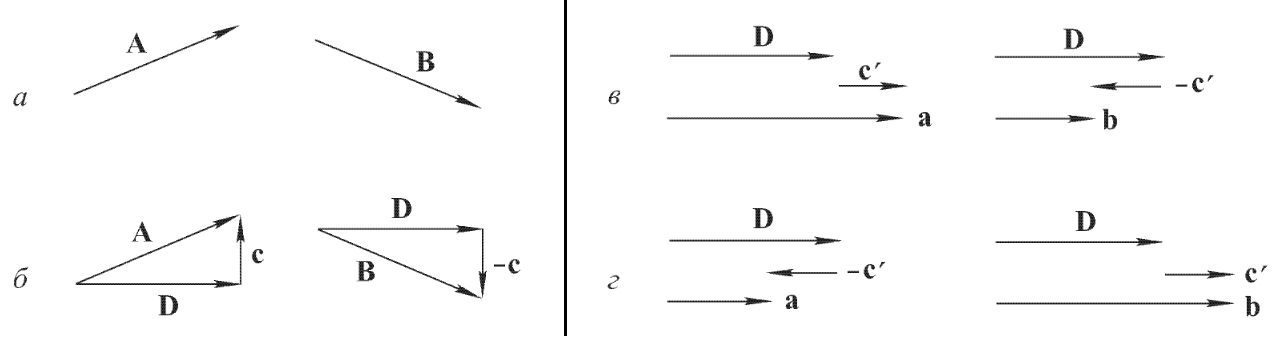
\includegraphics[width=0.65\textwidth]{figures/59_1.png}
    \caption{Метод фазового контраста}
    \label{fig:pfc59}
\end{figure}
Если повернуть $\vc{c}'$ и $\vc{c}$ на $\pi/2$, оставляя неизменным $\vc{D}$, то можем получить \textit{позитивный фазовый контраст} (в) и негативный фазовый контраст (г). 



\textbf{Реализация}. Прежде всего необходимо пространственно разделить волновые поля, представленные веткорами $\vc{c}$ и $\vc{D}$. Полное колебание имеет постоянную амплитуду на протяжении всей реешетки  и изображается вектором $\vc{D}$, оно даёт в фокальной плоскости центральный максимум, и только. 

Другое колебание представляется периодической функцией принимающую значения от $-\vc{c}$ до $\vc{c}$ на соседних участках, в среднем ноль, так что возбуждает только боковые максимумы, таким образом в фокальной плоскости объектива оба колебания окажутся пространственно разделенными. 

Поставив на пути либо центрального максимума, либо всех боковых максимумов прозрачную плоскопараллельную фазовую пластинке нужной тощины, можно ввести разность фаз в $\pi/2$ и так осуществить фазовый контраст. 


Стоит заметить, что раньше полная энергия на участках решётки была $2(D^2 + c^2)$, а после повтора $\vc{c}$ и $-\vc{c}$ энергия становится $(D+c)^2 + (D-c)^2$, то есть сохранятся, но перераспределяется. 





